
\section{System design} \label{sec:systemDesign}
%\hldone{Done}
The Rehab-Exos is an active robotic exoskeleton (\figurename \ \ref{fig:rehabexos1}) which is designed with the idea to be compact, easily reconfigurable and to have a good trade-off between transparency and force replication.
It was conceived for rehabilitation applications and it is designed in such a way to generate controlled contact forces/torques not only at its end-link handle, but also at  intermediate links. When the user is wearing the device he can control the full force interaction with the exoskeleton and guide/be guided involving all articulations of the arm (wrist, shoulder, elbow). 
The physical interaction between user and exoskeleton is monitored by the joint torque sensors which performances depend on several design and implementation aspects that are addressed in subsection \ref{subsec:DesignTorqueSensor}.
%%%%%%%%%%%%%%%%%%%%%%%%%%%%%%%%%%%%%%%%%%%%%%%%%%%%%%%%%%%%%%%%%%%%%%%%%%%%%%%%%%%%%%%%%%%%%%%%%%%%%%%%%%%%%%%%%%%%
%%%%%%%%%%%%%%%%%%%%%%%%%%%%%%%%%%%%%%%%%%%%%%%%%%%%%%%%%%%%%%%%%%%%%%%%%%%%%%%%%%%%%%%%%%%%%%%%%%%%%%%%%%%%%%%%%%%%
\subsection{Mechanical design of the Rehab-Exos} 
%\hldone{Done}
\label{subsec:mechanicalDesign}
As depicted in \figurename \ \ref{fig:rehabexos1} and in \figurename \ \ref{fig:rehabexosSchema}, the exoskeleton has a serial architecture isomorphic with the human kinematics that comprises: a shoulder joint  fixed in space and composed by three active joints $J_1$, $J_2$ and $J_3$; an active elbow joint $J_4$; and a passive revolute joint $J_5$ allowing for wrist prono/supination.  For a more detailed description of both Rehab-Exos and actuation groups, the reader can refer to \cite{vertechy2009development}.
%\begin{figure}[htb]
%	\centering
%	\subfigure[Exoskeleton kinematics]{\includegraphics[width=0.49\columnwidth]{\figpath{exos1}}\label{fig:exos_kinematics}}
%	\subfigure[CAD section of the joint actuator ]{\includegraphics[width=0.49\columnwidth]{\figpath{JointActuator}}\label{fig:exos_actuator}}
%	\caption{The Rehab-Exos CAD model showing overall kinematics and actuator structure}
%\end{figure}
\begin{figure}[]
	\centering
	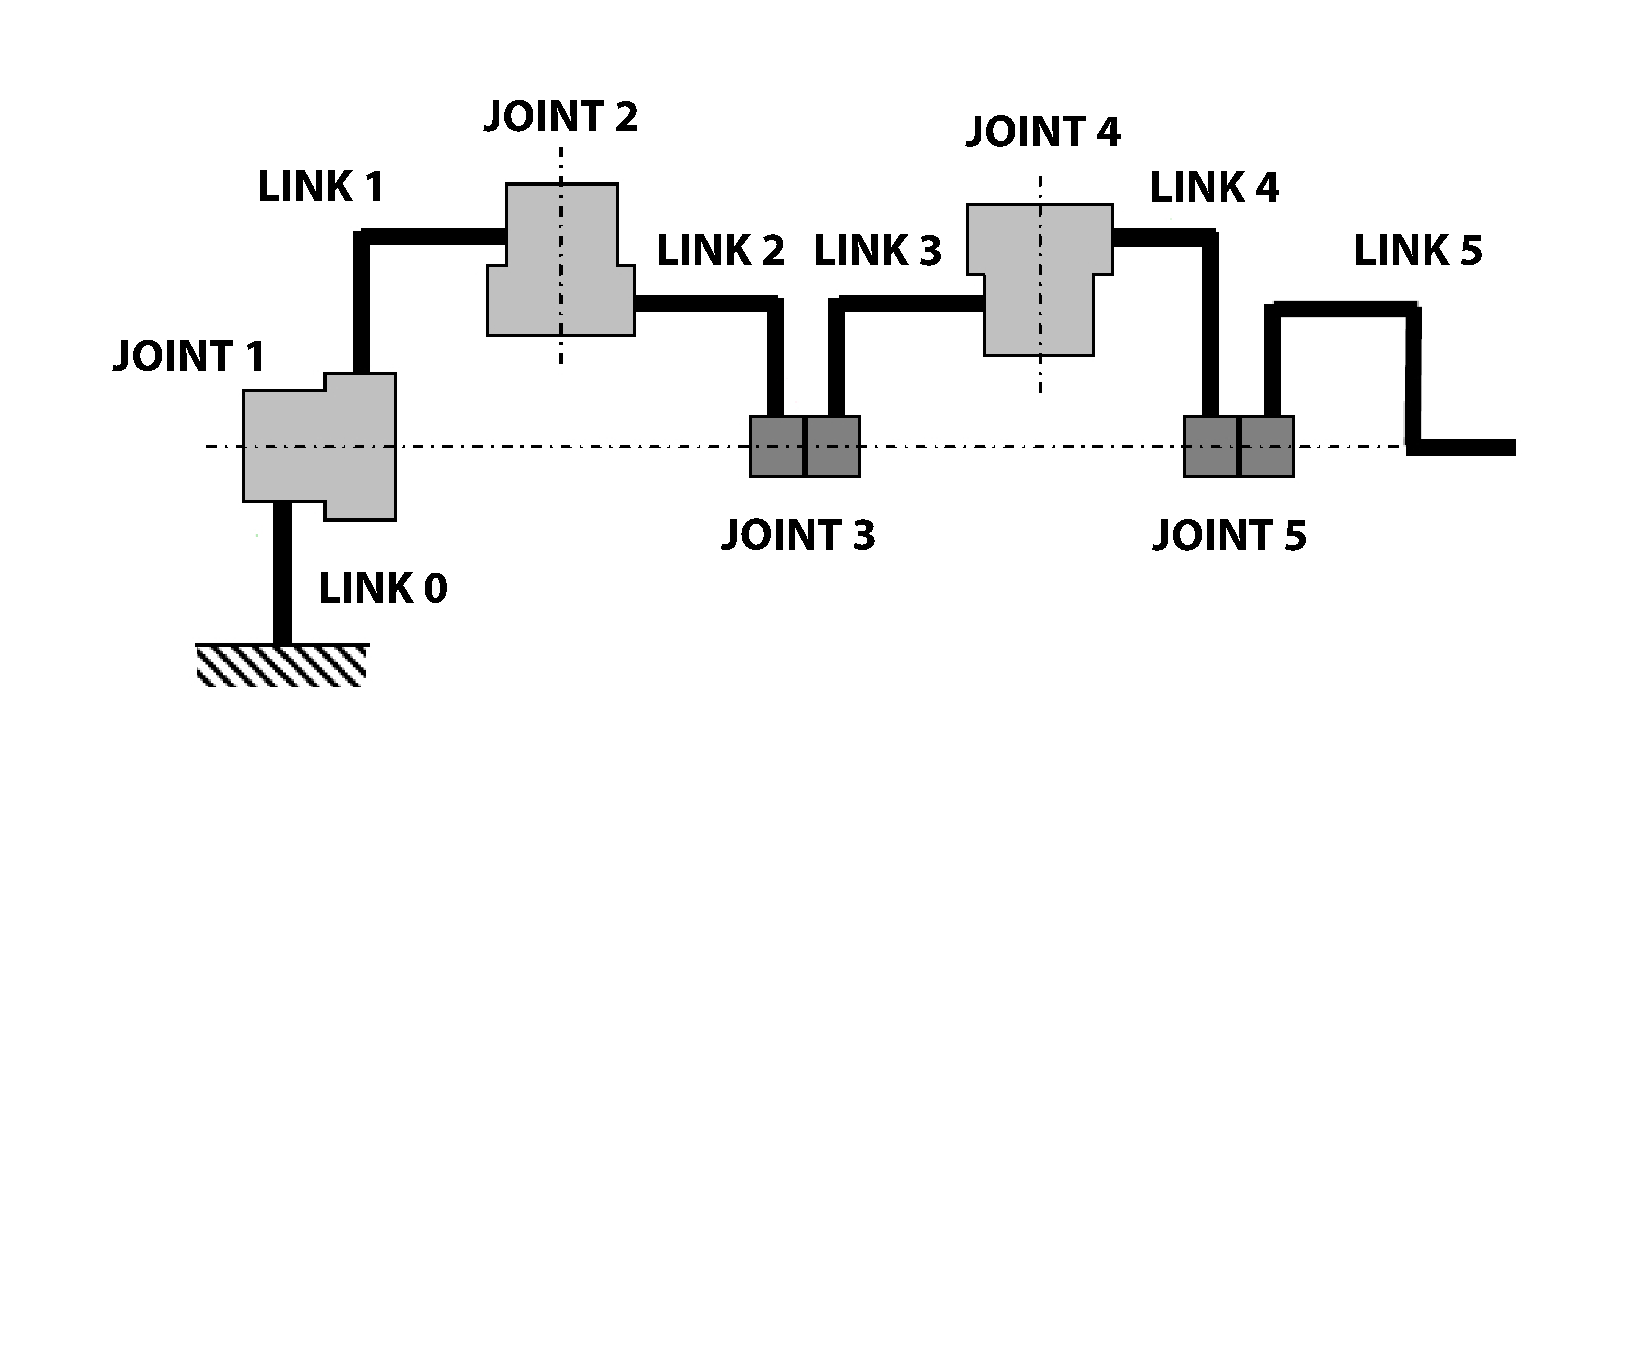
\includegraphics[width=0.9\columnwidth]{SchemaExos}
	\caption{A schematic representation of the Rehab-Exos exoskeleton.}
	\label{fig:rehabexosSchema}
\end{figure}
%
%
\begin{figure}[]
	\centering
	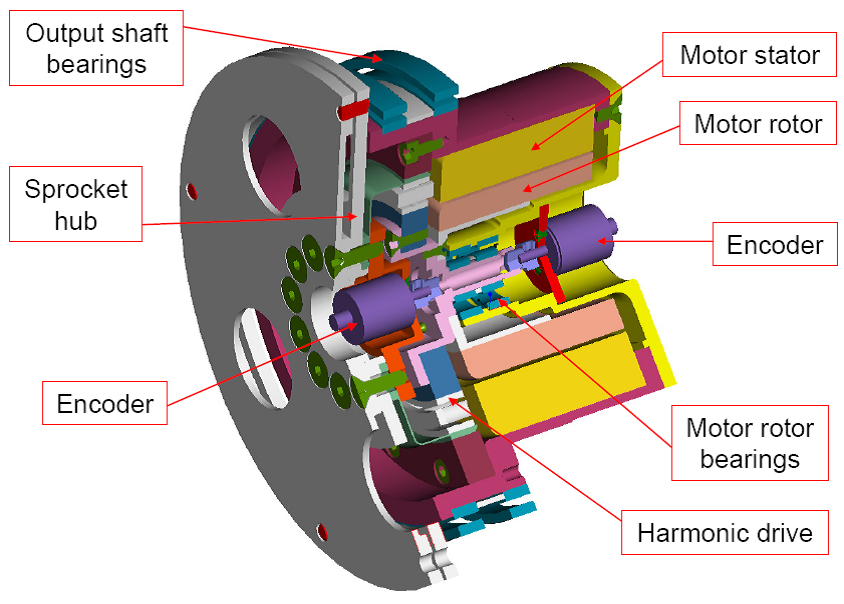
\includegraphics[width=0.7\columnwidth]{JointActuator}
	\caption{CAD section of the $J_1$, $J_2$ and $J_4$ joint actuator of the Rehab-Exos.}
	\label{fig:exosActuatorCAD}
\end{figure}
%
\par The three joints $J_1$, $J_2$ and $J_4$ of the exoskeleton are motorized through identical actuation groups. Each joint features a custom-made frame-less brush-less torque motor integrating a compact Harmonic Drive (HD) component set. The actuator provides a joint output torque equal to $150\ Nm$ with an overall weight equal to $3.7\ Kg$ and a motor shaft inertia reduced to the joint output shaft $Jm = 3.7\ Kgm^2$. The Harmonic Drive performs a reduction equal to 100:1. Due to the adopted mechanical components, the joints feature limited back-drivability at motor power-off and limited mechanical complexity to ease maintenance as well as reduce costs. A CAD section of the $J_1$, $J_2$ and $J_4$ joints is depicted in \figurename \ \ref{fig:exosActuatorCAD}.
Joint $J_3$ is characterized by a tendon transmission that is used to transmit the actuation torque through an open semi-circular guide. More detail on the joint $J_3$ can be found in \cite{vertechy2009development}.

\subsection{Design aspects of the strain gauge based torque sensor}
%\hldone{Done}
\label{subsec:DesignTorqueSensor}
The three joints $J_1$, $J_2$ and $J_4$ have a torque sensor featuring a four-spoke-shape geometry. 
Despite further augmenting the actuation group compliance, the availability of joint-torque sensors enables for multi-contact force control at multiple points distributed over the links and, additionally, makes it possible: 1) to close a stable high-bandwidth torque inner loop around each joint which is weakly affected by robot link variable inertia; 2) to suppress robot vibrations produced by the inherent transmission compliance (Harmonic Drive); 3) to reduce internal disturbance torques caused by actuator and reducer (for instance friction losses, actuator's torque ripples and gear teeth wedging actions); to measure externally applied forces/moments and complex non-linear dynamic interactions between joints and links.
\par The sensor consists of two fully balanced strain gauge bridges placed on different beams of the spoke, which is located at the joint output shaft. 
%
%
\begin{table}[t]
	\renewcommand{\arraystretch}{1.3}
	\caption{Characteristic dimensions of the torque sensor}
	\label{tab:sensorDimension}
	\centering
	\begin{tabular}{c c}
		\hline \hline
		\bfseries Dimension & \bfseries Value [$mm$] \\
		\hline
		R & 78 \\
		r & 38 \\
		L & 24 \\
		a & 4 \\
		round radius & 2 \\
		\hline \hline
	\end{tabular}
\end{table} 
%
\begin{figure}[]
	\centering
	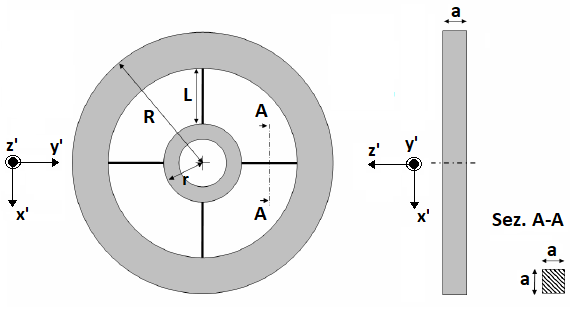
\includegraphics[width=0.7\columnwidth]{sensorDimensions}
	\caption{Characteristic dimensions of the torque sensor.}
	\label{fig:sensorDimensions}
\end{figure}
%
The sensor is made by AISI 630 steel, an harmonic steel exhibiting yield strength of 1950 MPa, Young's modulus of 196 GPa and has been dimensioned to exhibit low weight and high sensitivity to axial moments.
The axial torsional stiffness of the sensor is $k_s = 30 \ kNm/rad$ and can be calculated as in \eqref{eqn:sensorStiffness}.
\begin{equation}
\label{eqn:sensorStiffness}
k_{s} = \frac{\tau}{\theta} = \frac{Ea^4(r+L(1-Q))}{3L^2(1/2-Q)}	
\end{equation}
where the adimensional parameter Q is given by
\begin{equation}
\label{eqn:adimensionalQ}
Q = \frac{3r+L}{6r+3L}	
\end{equation}
where, according to \figurename \ \ref{fig:sensorDimensions}, $R$ is the radius of the external sensor ring, $r$ is the radius of the internal sensor ring, $L$ is length of the beams and $a$ is the side length of the beam section.
The characteristic dimensions of the sensor are reported in \tablename \ \ref{tab:sensorDimension}.
Moreover, the overall joint torsional stiffness reduced to the joint output shaft is $k = 11.38\ kNm/rad$.
\par The position of the strain gauges on the beam is a trade-off: if they were positioned in the middle of the beam the sensor sensitivity would be low, on the contrary, if they were positioned near the extremities the sensor reads would be affected by the non-linearities of the rounds of the beam. The selected distance from the extremities was $p = 1/8 \ L = 3 \ mm$.
To estimate the strain of the beam in a given point with distance $p$ from the inner ring under a certain axial torque $\tau$, the normal tension $\sigma_p$ that acts on that point $p$ needs to be computed as
\begin{equation}
\label{eqn:normalTensionOnBeam}
\sigma_p = \frac{3\tau((1-Q)L-p)}{2a^3((1-Q)L+r)}	
\end{equation}
and then the strain follow as 
\begin{equation}
\label{eq:strainEq}
\epsilon_A= \frac{\sigma}{E}
\end{equation} 
where $E$ is the Young's modulus.
\par Theoretically, i.e. using \eqref{eq:strainEq}, at $3 \ mm$ from the inner ring and under an axial torque of $120 Nm$,  a maximum strain of $2.7*10^-3 \ m$ is obtained.
The same test has been conducted using a FEM software tool (Ansys\textregistered) because the surface of the strain gauge is not negligible compared to the beam one (see \figurename \ \ref{fig:strainGaugeDeformation}) obtaining a maximum strain of $1.98*10^-3 \ m$.
The strain of each strain gauge when a $1 \ Nm$ load is applied can be shown in \tablename \ \ref{tab:sensorStrain}.
\begin{table}[]
	\renewcommand{\arraystretch}{1.3}
	\caption{Strain of the 4 strain gauges}
	\label{tab:sensorStrain}
	\centering
	\begin{tabular}{c c c c}
		\hline \hline
		\bfseries Probe 1 [m] & \bfseries Probe 2 [m] & \bfseries Probe 3 [m] & \bfseries Probe 4 [m]\\
		\hline
		1.65e-5  & -1.33e-5 & -1.91e-5 & 2.2546e-5\\
		\hline \hline
	\end{tabular}
\end{table} 
%
\par An important characteristic of the torque sensor is the sensitivity to non-axial moments, thus an experimental test has been conducted to compute the sensitivity, i.e. a predetermined non-axial torque has been exerted on the sensor in 4 configurations (angle) of the sensor.
Experimental results are reported in \tablename \ \ref{tab:sensorNonAxialResults} and the sensitivity is equal to
\begin{equation}
S_S=\frac{C_{mis}}{C_S}=0.067
\label{eq:sensitivityToNonAxLoad}
\end{equation} 
%
\begin{table}[]
	\renewcommand{\arraystretch}{1.3}
	\caption{Sensor reads to non-axial moments}
	\label{tab:sensorNonAxialResults}
	\centering
	\begin{tabular}{cc}
		\hline \hline
		\bfseries Applied Torque [Nm] & \bfseries Sensor reads per angle [Nm]\\
		$\;$ &	\begin{tabular}{cccc} $0^\circ$   & $45^\circ$ & $90^\circ$ & $180^\circ$ \end{tabular} \\
		\hline
		32 & \begin{tabular}{cccc} 1.6 & 2.4 & 2.2 & 2.3 \end{tabular} \\
		64 & \begin{tabular}{cccc} 2.9 & 4.8 & 4.4 & 4.4 \end{tabular} \\
		96 & \begin{tabular}{cccc} 4.5 & 7.5 & 6.9 & 6.9 \end{tabular} \\
		\hline \hline
	\end{tabular}
\end{table} 
The sensitivity to non-axial moments is relatively high compared to one mentioned in \cite{kashiri2017sensor}. %This non-ideal and non-linear characteristic were not found in the initial test-rig, instead non-axial loads are there in the multi-link mounted exoskeleton. 
%Despite the presence of the ball bearings, two factors influence the sensor readings. The first factor is the way the mechanical parts are assembled (assembly errors), the second is the non-axial loads influence on the sensor readings. 
\par The reason of these results has been investigated and two causes (or a combination of them) have been proposed. The first cause of error could be a strain gauges mounting misalignment. The second cause could be an excessive deformation of the sensor due to the non-axial moments. 
About the first hypothesis, the sensitivity of the strain gauges to non-axial load $C_S$ (when a flexible model of the HD is considered) due to strain gauges misalignment can be modeled as
\begin{equation}
S_{misal}= k_s \cdot (k_{ex} \cdot e_x + k_{e\theta} \cdot e_{\theta})
\label{eq:sensitivityMisalignment}
\end{equation}
where $k_s$ is a scaling factor equal to $7.87e^{-3}$, $k_{ex}$ is the sensitivity to linear mounting misalignment  equal to $3$, $k_{e\theta}$ is the sensitivity to angular mounting misalignment equal to $2.3$, whereas $e_x$ and $e_{\theta}$ are the positional and angular misalignment errors respectively (see \figurename \ \ref{fig:strainGaugeMisalignment}). Equation \eqref{eq:sensitivityMisalignment} and the measured sensitivity of 0.067 lead to a misalignment errors of millimeters and decades of degree, but these values are over the actual misalignment the installation operator may have introduced as can be seen in \figurename \ \ref{fig:strainGaugeParticular}.
%
\begin{figure}[]
	\centering
	\subfigure[]{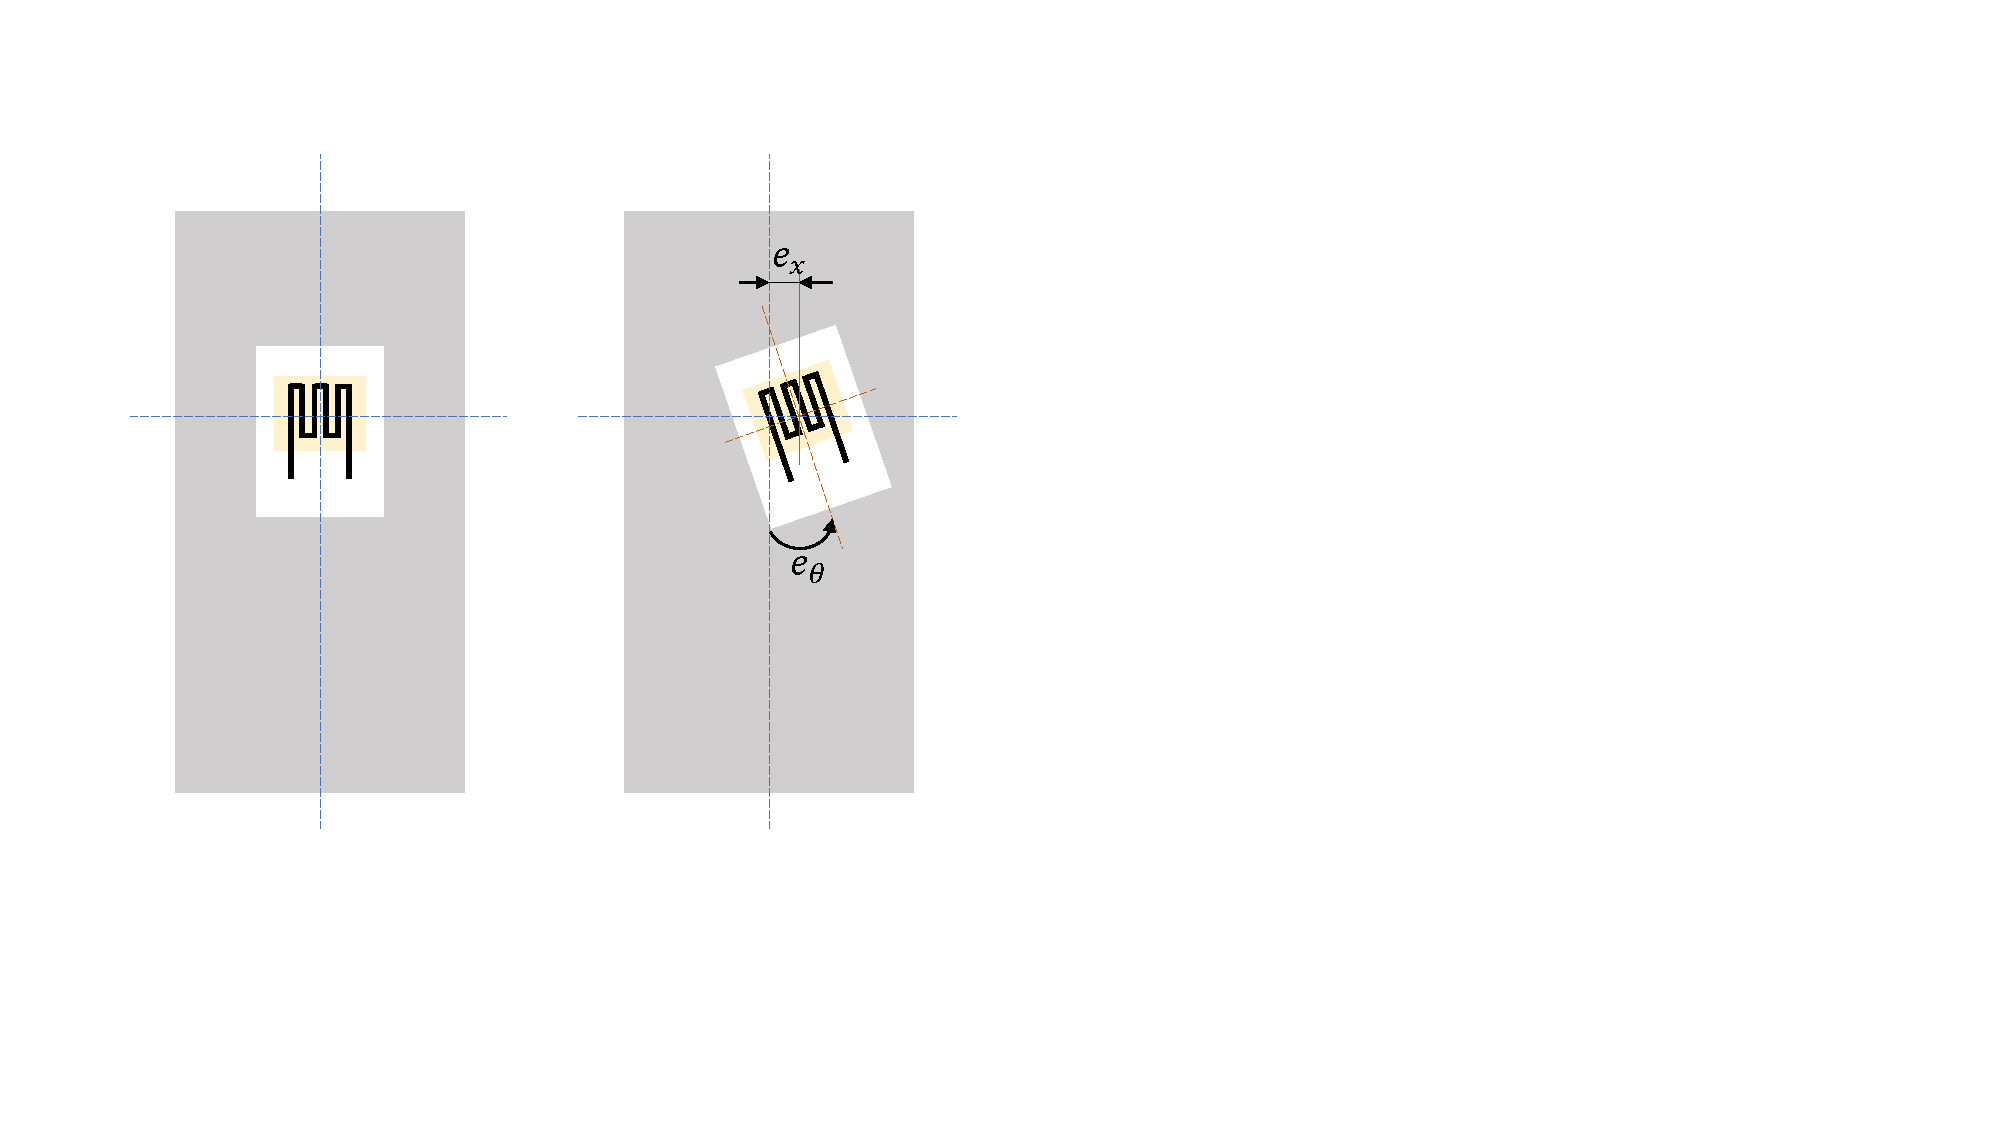
\includegraphics[height=0.35\columnwidth]{erroreMontaggioSensore} \label{fig:strainGaugeMisalignment}}
	\subfigure[]{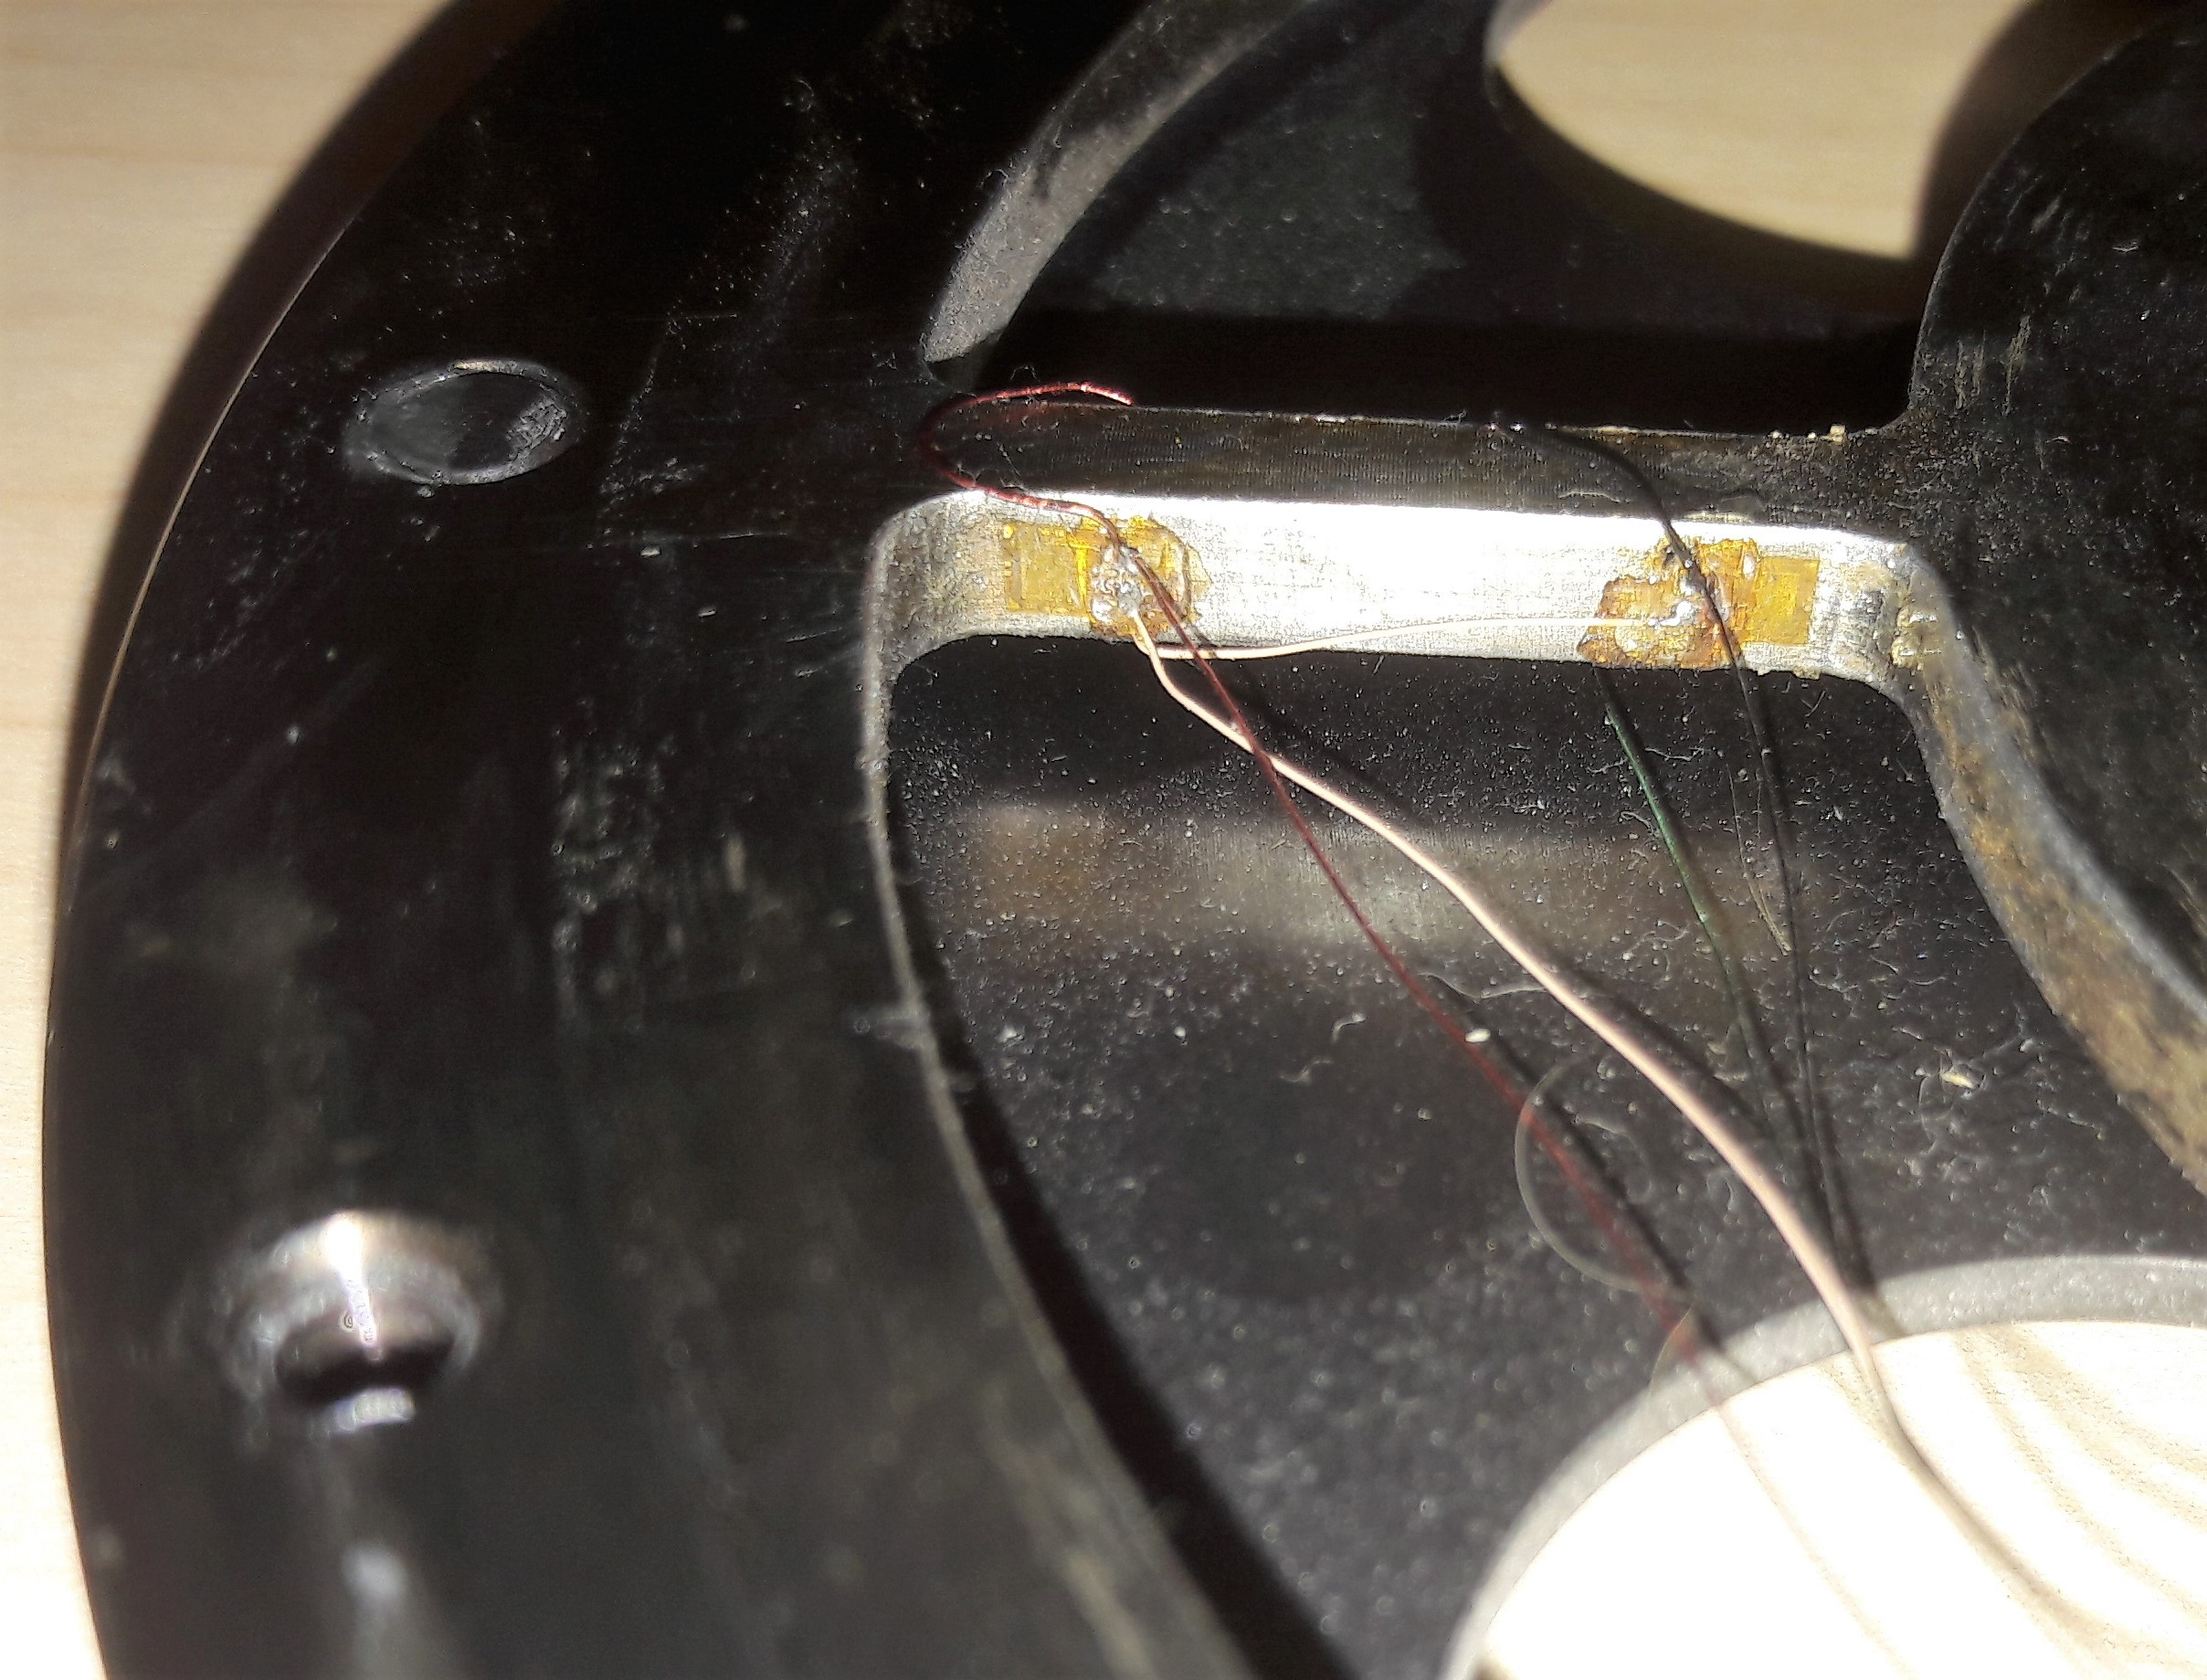
\includegraphics[height=0.32\columnwidth]{strainGaugeParticular.jpg} \label{fig:strainGaugeParticular}}
	\caption{A possible cause of high sensitivity to non-axial load is the strain gauges's mounting misalignment. The linear displacement $e_x$ and the angular one $e_{\theta}$ are highlighted in (a). A detail of the mounted strain gauges on the torque sensor in (b).} 
\end{figure}

About the second hypothesis it is worth to notice that the sensor from a structural point of view is in series to the HD and this series is in parallel with a couple of bearings. This parallel chain composes a hyper-static system (see \figurename \ \ref{fig:schemaGiuntoEMolle}), therefore the excessive sensitivity may be due mounting misalignment of the mechanical parts of the chain. 
%
\begin{figure}[]
	\centering
	\subfigure[]{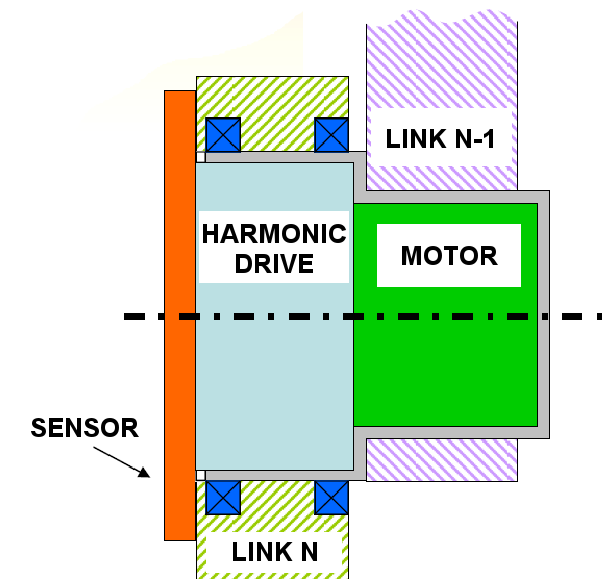
\includegraphics[width=0.49\columnwidth]{schemaGiuntoMod}\label{fig:schemaLinkGiuntoSens}}
	\subfigure[]{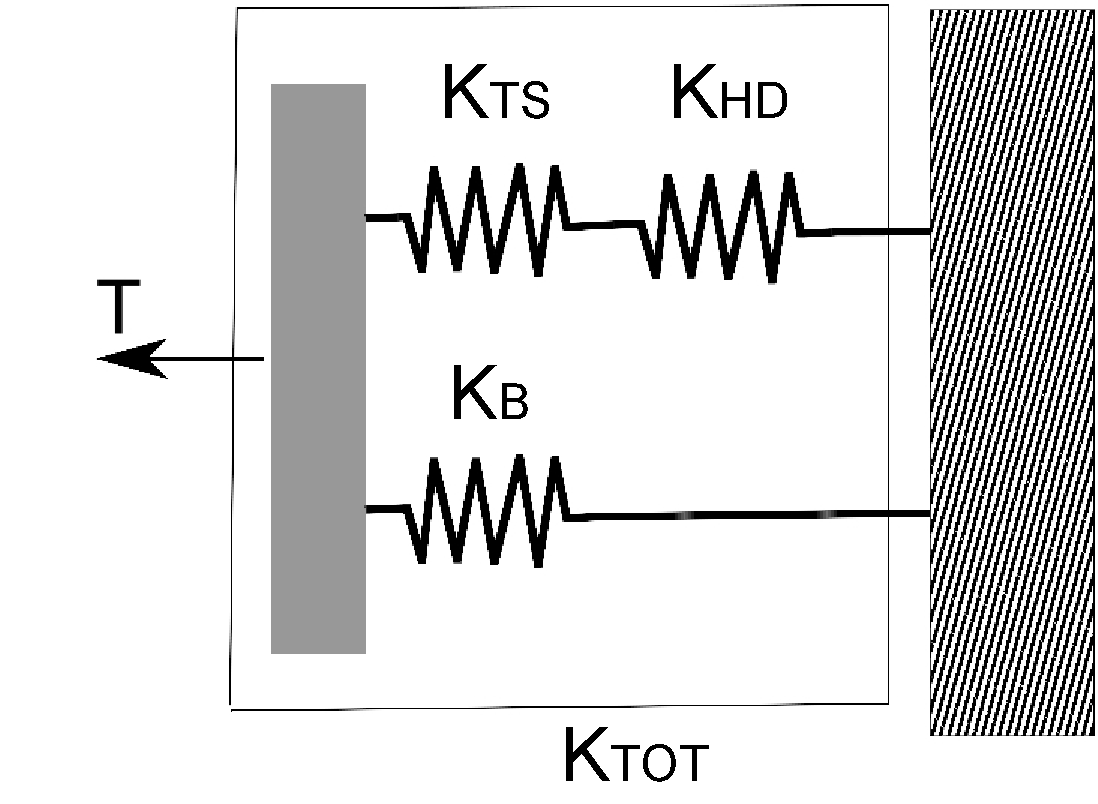
\includegraphics[width=0.49\columnwidth]{schemaMolle.pdf}\label{fig:schemaMolle}}
	\caption{In a), the schematic representation of the joint. The torque sensor is a series elastic element between the motor and the link n. The torque sensor is not structural and has been designed to transmit only axial torque. In b), the kinematic chain of the joint to non-axial loads. $K_{TS}$ and $K_{HD}$ are the stiffness of the torque sensor and of the Harmonic Drive to non-axial load respectively, whereas $K_B$ is the bearing stiffness.}
	\label{fig:schemaGiuntoEMolle}
\end{figure}
%
\par For the study of the hyper-static system a linear  elastic behavior of the system parts were supposed and the system response at non-axial moments was modeled as a mono-dimensional model as in \figurename \ref{fig:schemaMolle}.
The overall joint stiffness to non-axial moments $K_{TOT}$ was experimentally evaluated, whereas the non-axial moment stiffness of the torque sensor $K_{TS}$ and of the HD $K_{HD}$ were computed via FEM analysis. The FEM results are depicted in \figurename \ \ref{fig:strainGaugeDeformation} and the stiffness values are reported in table \tablename \ \ref{tab:nonAxialStiffness}.
%
\begin{figure}[]
	\centering
	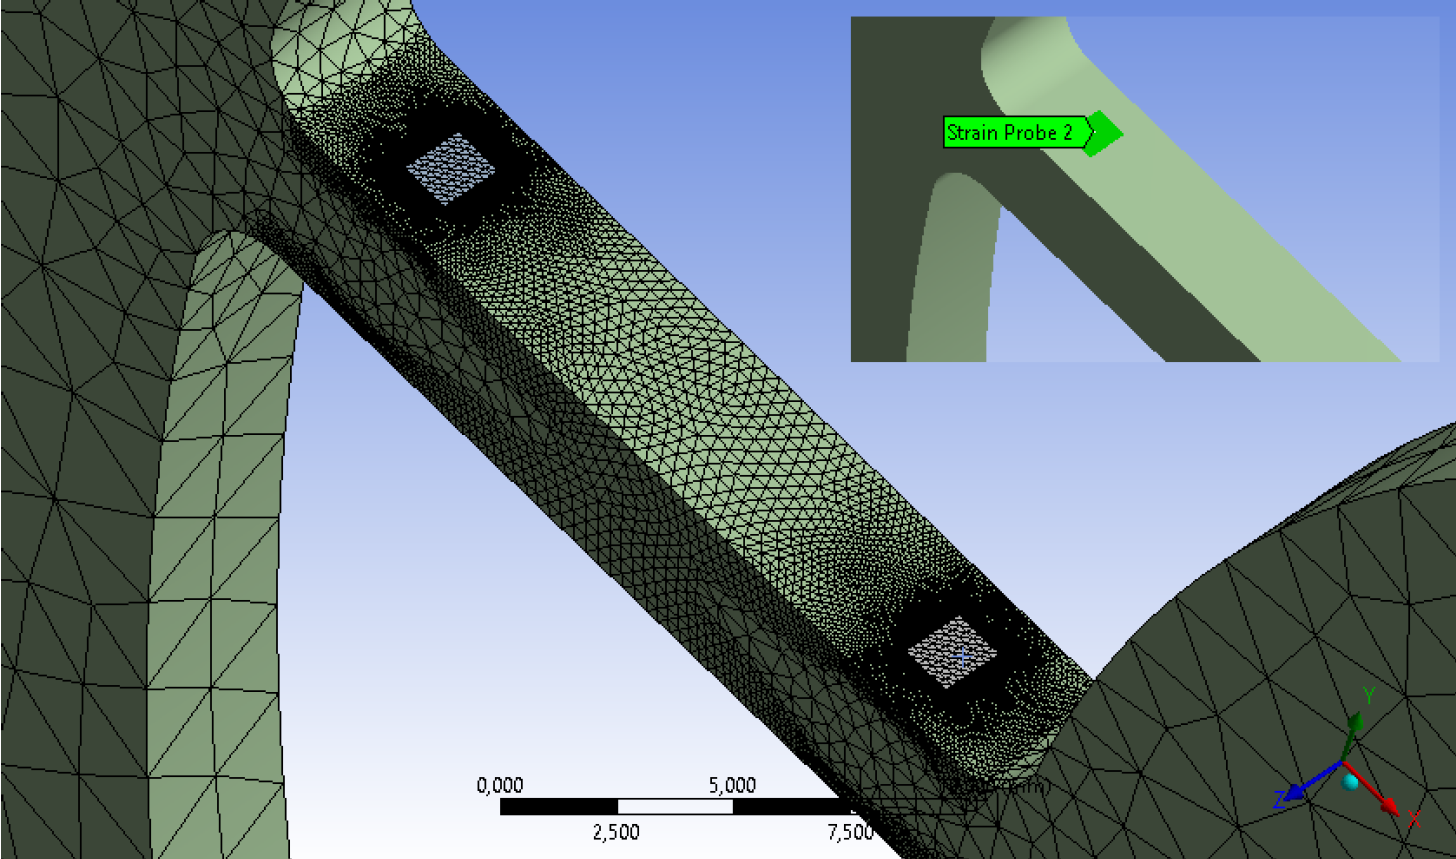
\includegraphics[width=0.7\columnwidth]{strainGaugeDeformation} 
	\caption{For the FEM analysis a more dense grid mesh for the zone of interest has been used. For each area the average strain along the radial direction has been computed.}
	\label{fig:strainGaugeDeformation}
\end{figure}
%
\begin{table}[]
	\renewcommand{\arraystretch}{1.3}
	\caption{Stiffness of the components}
	\label{tab:nonAxialStiffness}
	\centering
	\begin{tabular}{c c}
		\hline \hline
		\bfseries Component & \bfseries Stiffness [kNm/rad]\\
		\hline
		$K_{TS}$  & 4.1\\
		$K_{HD}$  & 0.4\\
		$K_{B}$   & 23.6\\
		\hline
		$K_{TOT}$   & 24\\
		\hline \hline
	\end{tabular}
\end{table}
%
%
\par A possible mounting misalignment of the hyper-static chain may be a collinear and/or concentric mounting misalignment between the sensor axis and the bearing axis. In this case, the HD works as an universal joint that connect the sensor (that is connected to the (n+1)-th link ) and the n-th link. The sensitivity to non-axial moments defined in equation \eqref{eq:sensitivityToNonAxLoad} and  the mechanical properties  in \tablename \ \ref{tab:nonAxialStiffness} lead to a theoretical mounting misalignment of about $0.5 \ mm$, but this value is not in agreement with the design tolerances and components data-sheets from which a misalignment of about $0.05 \ mm$ results in the worst case.
%
%The internal joint-torque sensor introduces controlled torsional compliance that is used at the same time to transmit joint torque actuation  from the motor to the link and to measure it. 
%The torque sensor is not structural and the mechanical transmission is parallel (see the scheme in \figurename \ \ref{fig:schemaLinkGiuntoSens}). The planar sprocket hub has been designed to be sensitive only to the torque along the motor axes exchanged between the motor on the link $n-1$ and the link $n$, while theoretically the torques along the other two axes are transmitted directly through the ball bearings between the link $n-1$ and the link $n$.
\par To summarize, unwanted sensor reads to non-axial load may be due to the combination of effects from sensor mounting misalignments and HD excessive deformation. 
\par In order to minimize this undesired effect the authors propose a method based on artificial neural networks (ANN) to characterize and compensate this non-linear behavior that results difficult to model.
%
%
Considering the ideal and linear sensor, the torque readings can be expressed as $\tau_s = k_v * v$, where $v$ is the measured voltage tension and $k_v$ is the torque sensor's voltage constant. In the real case it be can written $\hat{\tau}_s = k_v * v + \delta\tau$, where $\delta\tau$ is the non-linear influence on the sensor readings due to the mounting and non-axial loads.
By experimental evidence, it's possible to assert that the term $\delta\tau$ varies in a non-linear way with respect the exoskeleton pose (joint angles) and load.
\par The mounting errors influence the torque readings non-linearly with respect to the joint angle, while the non-axial torques depends in part on the interaction with human and in part on the dynamics and gravitational torques acting on the considered joint.
%\begin{figure}[htb]
%	\centering
%	\includegraphics[width=0.55\columnwidth]{\figpath{schemaGiuntoMod}}	
%	\caption{}
%	\label{fig:schemaLinkGiuntoSens}
%\end{figure}
%
\begin{figure}[]
	\centering
	\subfigure[]{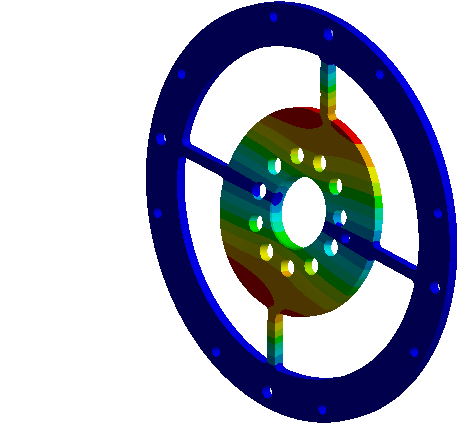
\includegraphics[height=0.4\columnwidth]{sensoreCarichiSpuri} \label{fig:sensoreCarichiSpuri}	}
	\subfigure[]{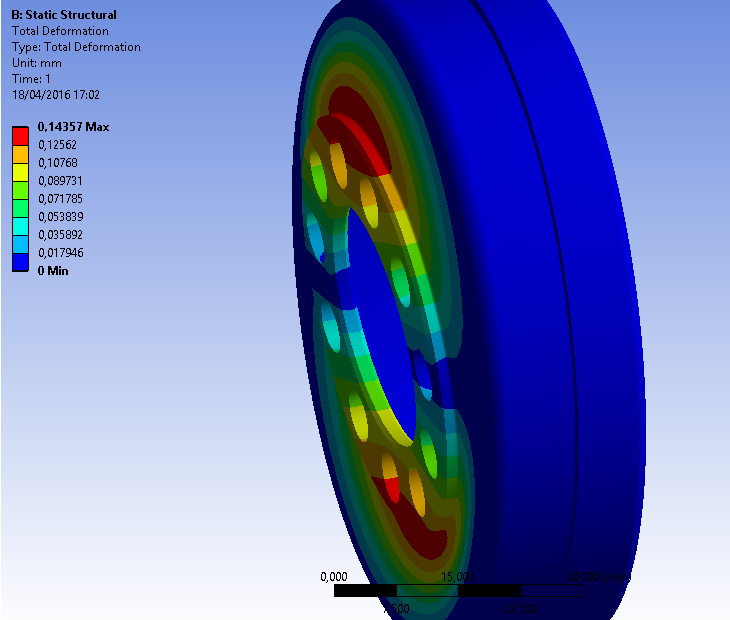
\includegraphics[height=0.4\columnwidth]{HDCarichiSpuri} \label{fig:HDCarichiSpuri} }
	\caption{The FEM analysis results of the torque sensor (a) and of the flexible spline (b) deformation under non-axial load.}
\end{figure}
%
%
For all the three sensors the $k_v$ constants have been experimentally evaluated. In order to minimize the effect of non-linear undesired term $\delta\tau$,  an ANN has been used. ANN is a mathematical approximation approach that is capable to infer non-linear behavior from experimental acquisitions. The ANN with 7 neurons in the hidden layer and sigmoid activation function are deputed to estimate the error on the basis of the 4 angles and load on each axis. The angular information is useful to infer the assembly error component, whereas for the load influence the gravitational torque has been used. 
\par To train the neural network the whole workspace has been partitioned in 414 target points. The torque sensor readings were acquired while the exoskeleton was holding the target position. For each joint, the training has been done using as input the 4 angles and the gravity torque that act on the joint (computed by model), and as output the residual value $\hat{\delta\tau} = G_i(\vect{\theta_m}) - k_v * v$, where $G_i$ is the gravity load on the i-th joint when the pose is given by the angle vector $\vect{\theta_m}$. The set of target points was divided in 3 parts: 70\% for the training set, 20\% for the validation set and 10\% for the test set. The regression value between the ANN output and the target points is 0.99.
The actual sensor torque estimation is given by $\bar{\tau}_s = k_v * v + \delta\tau(\vect{\theta_m},G_i)$, and a scheme of this estimation is shown in the \figurename \ \ref{fig:NN_schema}.
\begin{figure}[]
	\centering
	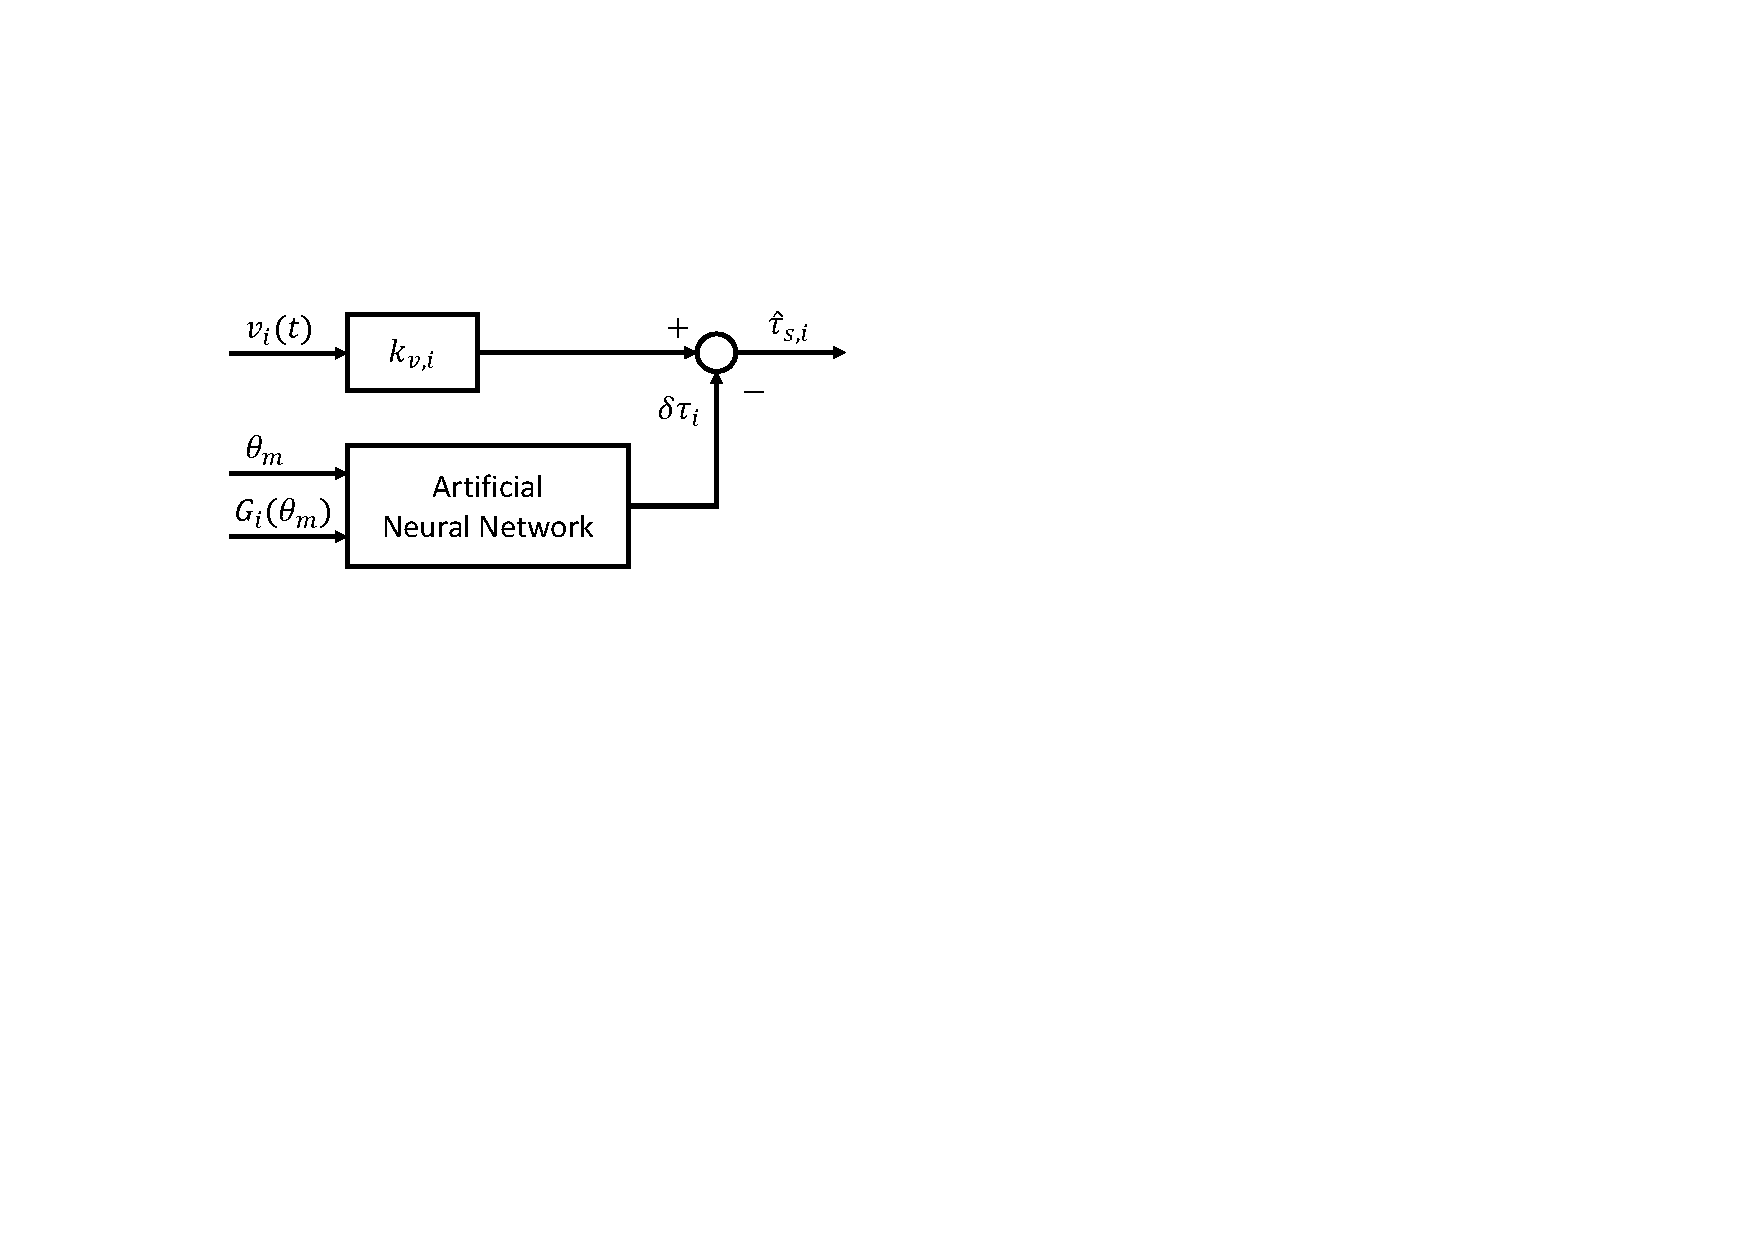
\includegraphics[width=0.7\columnwidth]{torqueEstimation}	
	\caption{The estimated sensor torque is obtained as the sum of sensor's reading and the predicted undesired non-linear term.}
	\label{fig:NN_schema}
\end{figure}
%\hl{QUi} As can be shown in the \figurename \ N, the introduction of the undesired term prediction induce a reduction in interaction force while a zero torque following control is implemented (see section N). Note that the force reduction is measured by the end effector force/torque sensor, while the  torque control use only the estimated torque using the sensor readings.
%%%%%%%%%%%%%%%%%%%%%%%%%%%%%%%%%%%%%%%%%%%%%%%%%%%%%%%%%%%%%%%%%%%%%%%%%%%%%%%%%%%%%%%%%%%%%%%%%%%%%%%%%%%%%%%%%%%%
%%%%%%%%%%%%%%%%%%%%%%%%%%%%%%%%%%%%%%%%%%%%%%%%%%%%%%%%%%%%%%%%%%%%%%%%%%%%%%%%%%%%%%%%%%%%%%%%%%%%%%%%%%%%%%%%%%%
\subsection{Control Hardware}
%\hldone{Done}
The control architecture of the Rehab-Exos is decentralized and based on the EtherCAT communication bus in order to guarantee both optimal signal to noise ratio in the acquisition of analogical signals, i.e. force sensors, and higher standards of safety.
The EtherCAT communication network consists of one master controller and four Ethercat Slave Controllers (ESC), one for each actuation joint.
The master controller is handled by Simulink Real-Time\texttrademark \ Operating System that executes the centralized control model at $2 \ kHz$ frequency.

Motors of the exoskeleton consist of three $170 \ VDC$ power supplied brush-less motors on the 1st, 2nd and 4th joint each one driven by programmable current driver and one $48 \ VDC$ power supplied DC motor on the 3th joint.  All of them are provided with one incremental encoder and one torque sensor.

Each ESC board is a custom control board featuring an up-to $72 \ Mhz$ ARM7 micro-controller, 4 14-bit DAC output interfaces (to set the reference of the current drives), 10 14-bit Analog-to-Digital Converter (ADC) channels (to acquire the torque signals through 2 Wheatstone full-bridge channels that are pre-amplified) and the EtherCAT ET1100 controller linking to double-port Ethernet interface.
%\begin{figure}[ht]
%	\centering
%	{\includegraphics[width=0.95\columnwidth]{\figpath{HWControlDiagram}}}
%	\caption{The decentralized control architecture}
%	\label{fig:ControlArchitecture}
%\end{figure}